\chapter{Radiodiagn\'ostico metab\'olico estudiado con simulaciones Monte Carlo}

El presente capítulo está dedicado a presentar muy brevemente las características básicas de las técnicas de radiodiagnóstico de tipo funcional. Se describe cómo éstas permiten recavar información de carácter metabólico para complemetar la información disponible en vista de realizar el diagnóstico en ámbito clínico. Se puntualizan los aspectos principales sobre cómo implementar técnicas de simulación Monte Carlo para estudiar este tipo de procesos de imaging.

\section{Im\'agenes funcionales para fisiolog\'ia metab\'olica}

Actualmente, la combinación de técnicas físicas sofistiadas y métodos de procesamiento digital de los datos obtenidos por las máquinas que adquieren las imágenes médicas es un campo que permite extraer una información que se sitúa más allá de la simple observación de las imágenes en las placas radiográficas o en los monitores diagnósticos. Las técnicas actuales permiiten, por medio de métodos digitales, proveer información precisa de la anatomía del área estudiada y obtener, a la vez, información funcional.

Para estudiar la funcionalidad subyacente se han utilizado técnicas como la tomografía por emisión de positrones (PET) o la tomografía por emisión simple de fotones (SPECT). Sin embargo, el dispositivo típico y más común para la detección de radiación en aplicaciones de medicina nuclear es la cámara gamma, en la modalidad indicada en la figura \ref{camgam}.

\begin{figure}
 \centering
 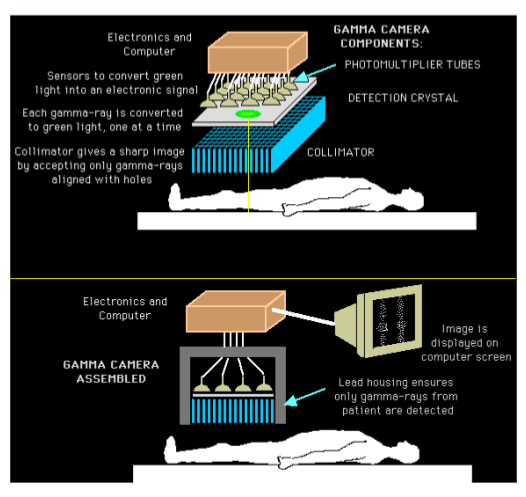
\includegraphics[width = .75\textwidth]{figures/cap9/camgam.png}
 \caption{Configuración para estudios en medicina nuclear utilizando cámara gamma.}
 \label{camgam}
\end{figure}

El principio básico de funcionamiento de la cámara gamma como equipamiento de imágenes de medicina nuclear es aprovechar la incorporación al paciente de moléculas que contienen algún átomo radioactivo y que, dependiendo del metabolismo será su distribución en el tiempo. Puede ser usada para tratamiento, como en el caso del $^{131}$I, que en dosis adecuadas se deposita en la tiroides y conformando un tejido de similar comportamiento (cáncer de tiroides) destruyendo sus células o puede usarse también para diagnóstico.

\section{Aplicaciones en C\'amara Gamma}

En términos técnicas, la cámara gamma consiste en un colimador, o blindaje calibrado, para que la radiación del radioisótopo a evaluar sólo pueda alcanzar el detector si ha realizado una trayectoria perpendicular al mismo; un detector de radiación por centelleo, que es un cristal en el que al incidir radiación emite luz, luego ésta es captada por un arreglo de fotomultiplicadores (sistemas electrónicos que transforman la luz en una corriente eléctrica); después del arreglo de fotomultiplicadores, un sistema electrónico realiza la detección contando y catalogando estos eventos para armar un mapa de distribución plano de la radiación frente al detector. La intensidad de la radiación detectada depende tanto de la distribución como de la atenuación que sobre la radiación realiza la parte del cuerpo del paciente que se interpone entre el punto donde se produjo un determinado evento y el detector.

La figura \ref{appcamgam} muestra esqumáticamente la constitución de la cámara gamma y el osbozo del trazado de rayos.

\begin{figure}
 \centering
 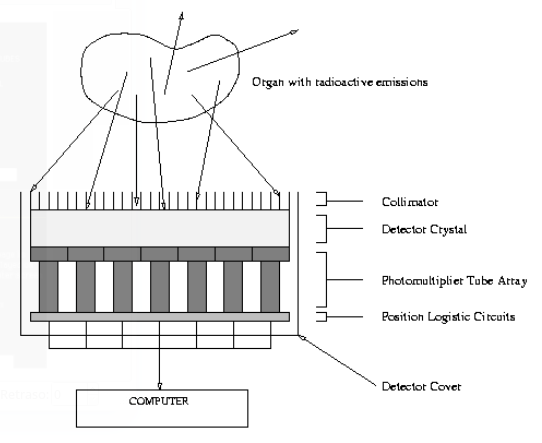
\includegraphics[width = .75\textwidth]{figures/cap9/appcamgam.png}
 \caption{Esquema de los componentes básicos de un detector tipo cámara gamma.}
 \label{appcamgam}
\end{figure}

Actualmente, estos sistemas además de permitir la adquisición de imágenes planas, pueden rotar alrededor del paciente obteniendo varias imágenes planares con las que, computadora por medio de un algoritmo matemático, genera cortes transversales, mejorando la relación señal a ruido, recuperando información perdida por atenuación y en general optimizando el diagnóstico.

Cada imagen de cámara gamma, así como una radiografía, brinda información bidimensional, pero pueden combinarse muchas imágenes tomadas desde distintas posiciones alrededor del paciente para obtener una imagen tridimensional, dando lugar a, por ejemplo, la técnica de Single Photon Emission Computed Tomography -SPECT. Esta imagen tridimensional puede después manipularse de manera digital para obtener secciones dimensionales del cuerpo en cualquier orientación requerida.